\section{Solution}

%----------------------------------------------------------------------------------------
%	PROJECT STRUCTURE SUBSECTION
%----------------------------------------------------------------------------------------
\subsection{Project Structure}
Project contains a core folder in HAL that contains task.h and task.c implementations and also IO which is a micro-controller connection abstraction.
\\\\
\centerline{
	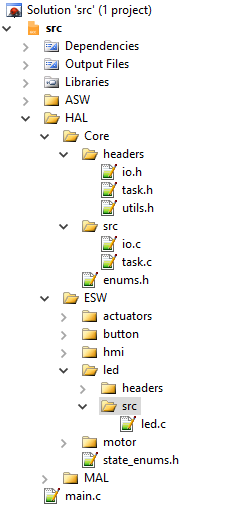
\includegraphics[width=0.5\textwidth]{solution/images/src.png}
}

%----------------------------------------------------------------------------------------
%	MAIN PROGRAM SUBSECTION
%----------------------------------------------------------------------------------------

\subsection{Main program flow}
\begin{enumerate}
	\item Global variable declarations.
	\item Tasks initialization
    \item Scheduler initialization and running
    \item Adding tasks to scheduler
	\item Start infinite loop (Controller life cycle)
\end{enumerate}

%----------------------------------------------------------------------------------------
%	PROTEUS SUBSECTION
%----------------------------------------------------------------------------------------

\newpage
\subsection{Circuit in Proteus}
I've connected 3 led of 3 different colors to micro-controller that will be turned on and off by task runner with different interval\\\\
\centerline{
	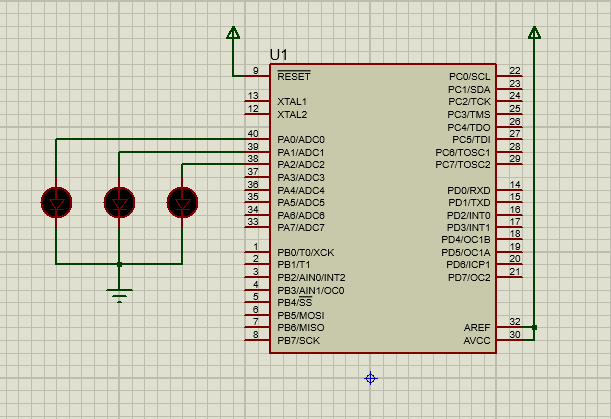
\includegraphics[width=1.0\textwidth]{solution/images/schematics.png}
}

%----------------------------------------------------------------------------------------
%	SIMULATION SUBSECTION
%----------------------------------------------------------------------------------------
\subsection{Simulation}
\centerline{
	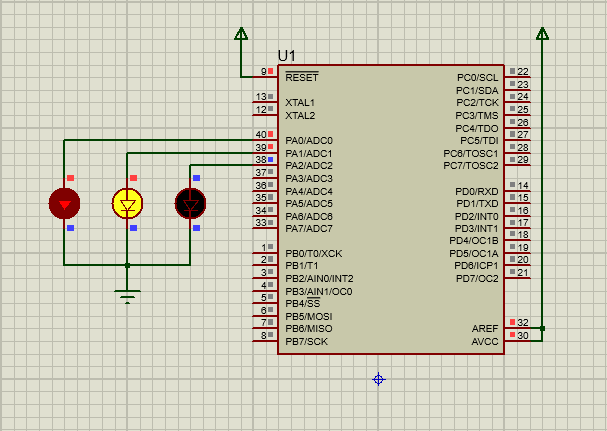
\includegraphics[width=1.0\textwidth]{solution/images/result.png}
}

